\chapter{Classification of Wikipedia articles}\label{experiments_chapter}
    This chapter describes and discusses the experiments that have been performed using the learning framework.
    
    Since I did not have enough computational resources to run a graph-based convolutional network on the entire multilingual graph of Wikipedia articles, I decided to use a simpler approach:
    \begin{enumerate}
        \item Build a multilingual graph of the categories.
        \item Use the learning framework together with a graph-based convolutional neural network to learn how to assign a soft label (probability distribution over classes) to each vertex of the multilingual graph.
        \item To classify an article, take all the categories it belongs to, take the average probability distribution over classes, and keep the class corresponding to the maximum value of the resulting probability distribution.
    \end{enumerate}
    The results are promising and can definitely improve by using the learning framework on the multilingual graph of the articles itself and by adding features to each vertex.
    \section{Building multilingual graphs}
        I have tried to experiment with Wikipedia multilingual graphs in order to study some of their properties. In particular, I wanted to answer the following questions:
        \begin{itemize}
            \item Does it make sense to exploit inter-language links between pages belonging to different Wikipedia editions in order to build a multilingual graph?
            \item How many are the ambiguities in the graph created with inter-language links? What are the causes of these conflicts?
            \item Are the predefined merging strategies useful? Are they able to solve conflicts? How do they behave compared to strategies proposed in other papers?
        \end{itemize}
        
        The experiments that follow are performed on four Wikipedia editions --- English, Italian, German and French --- and are based on their category graphs. Data come from the dump dated January 1st 2019.
        
        \subsection{Strongly connected components}
            First, I used the builder described in section \ref{categorygraphbuilder} to automatically build the category graph of each Wikipedia edition. All the hidden and administration categories were removed. Also, redirects were removed: categories that redirect to other categories were simply ignored, and categories that are target of redirect categories inherited their relationships. Then, I built a graph where vertices were the remaining categories belonging to the four Wikipedia editions and the edges were the inter-language links between them.
        
            \begin{figure}
                \centering
                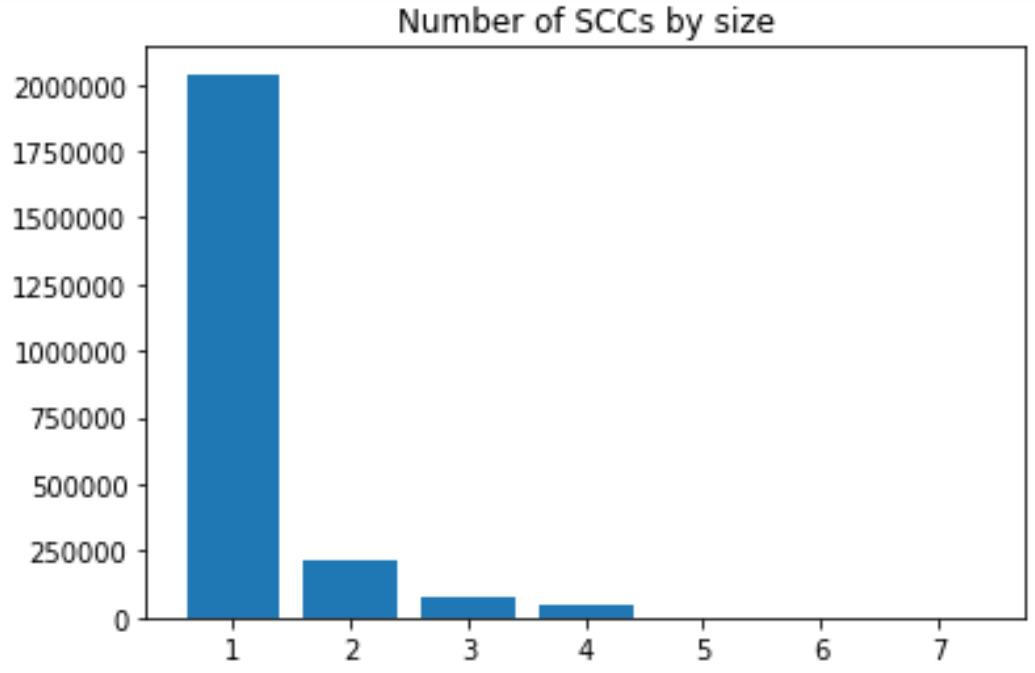
\includegraphics[width=0.6\textwidth]{images/scc_by_size.PNG}
                \caption{Number of strongly connected components in the Wikipedia multilingual graph built using categories belonging to English, Italian, German and French editions, and their related inter-language links. Data come from the dump dated January 1st 2019.}
                \label{scc_by_size}
            \end{figure}
            
            \begin{figure}
                \centering
                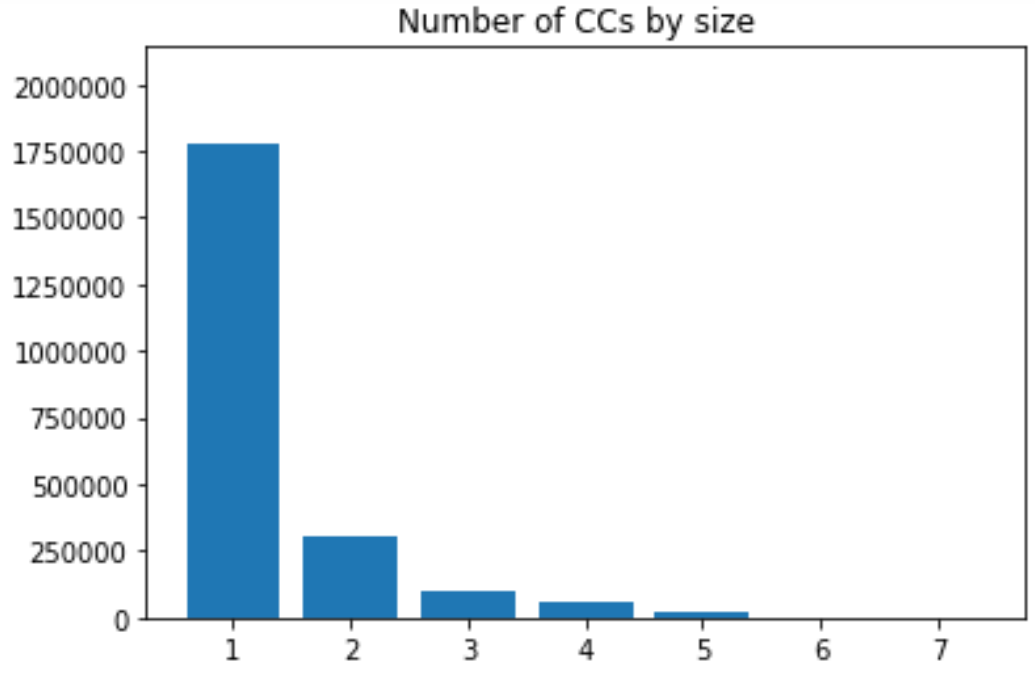
\includegraphics[width=0.6\textwidth]{images/cc_by_size.PNG}
                \caption{Number of connected components in the Wikipedia multilingual graph built using categories belonging to English, Italian, German and French editions, and their related inter-language links. Data come from the dump dated January 1st 2019.}
                \label{cc_by_size}
            \end{figure}
        
            Figure \ref{scc_by_size} is an histogram showing the number of strongly connected components of such graph. One can easily notice a couple of things from this figure:
            \begin{itemize}
                \item The number of conflicts is probably very small. Indeed, an ambiguity occurs only when multiple pages in the same language edition are connected via pages in other language editions, meaning that a corresponding multilingual page would have more than one page per language. Since the graph has been built using only four languages, conflicts are not likely to occur because basically all the strongly connected components have less than four nodes.
                \item The fact that most categories of the Wikipedia multilingual graph belong to a single-node strongly connected component means that very few nodes can be merged if one uses only inter-language links.
                
                This result is not caused by the use of strongly connected components. Indeed, as you can see in figure \ref{cc_by_size}, it is confirmed also when connected components are used in place of strongly connected components.
            \end{itemize}
        
            The fact that most of the components are formed by a single node can mean two things: either there are missing inter-language links or categorization systems provided by different Wikipedia editions differ a lot between them. I have briefly investigated this fact by analyzing a sample of 50 random single-node strongly connected components. Specifically, I have focused on Italian and English editions only, since they are the only languages I am fully comfortable with. To the best of my knowledge, there were no missing inter-language links between these two editions --- i.e., I was not able to find a single-node strongly connected component with an associated translation in a different language. Though the sample was small, I am convinced that the quality of editions I have analyzed is high, and that the fact that most components are formed by a single node is caused by differences in the categorization system. This does not necessarily mean that a topic is covered only in a single language edition, but simply that different communities have chosen to categorize pages in a different way. For example, compared to the English Wikipedia, the Italian one does not divide \textquote{Meteorologia} --- i.e., \textquote{Meteorology} --- into its various branches (for example, \textquote{Tropical meteorology} or \textquote{Marine meteorology}), but it still provides basically all the articles contained in the English Wikipedia: in this case, the English categorization system is more specific and detailed with respect to the Italian one, but the topics covered by the two editions are substantially identical.
        \subsection{Applying the merging strategy}
            \begin{figure}
                \centering
                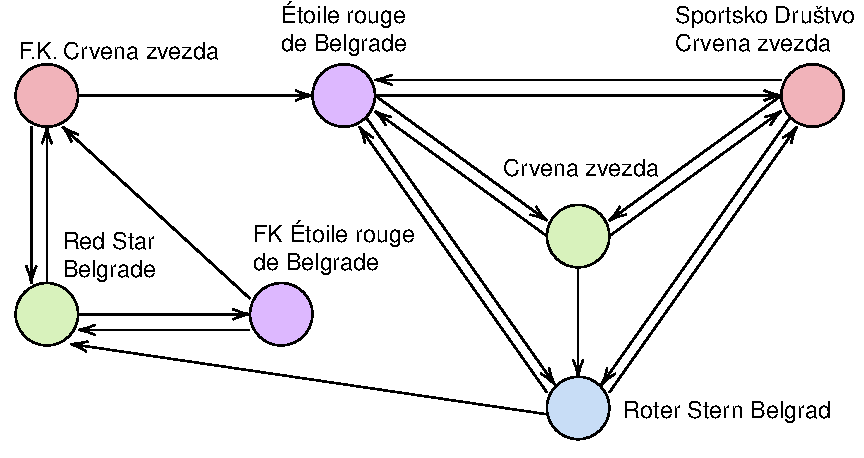
\includegraphics[width=\textwidth]{images/red_star.pdf}
                \caption{A typical ambiguity of the Wikipedia multilingual graph built with categories and inter-language links.  Different colors represent nodes belonging to different Wikipedia editions: green is used for English, red for Italian, blue for German and purple for French. Data come from the dump dated January 1st 2019. Here the confusion is caused by the fact that both the football club from Belgrade (\textquote{Fudbalski klub Crvena zvezda}) and the multi-sport club from Belgrade (\textquote{Sportsko društvo Crvena zvezda}) are sometimes simply called \textquote{Red Star}.}
                \label{red_star}
            \end{figure}
            
            I also applied the predefined merging strategy described in section \ref{merging_strategy} to the ambiguities found in the multilingual graph. Typical conflicts and ambiguities that can occur are shown in figure \ref{red_star} and \ref{istanbul}.
        
            \begin{figure}
                \centering
                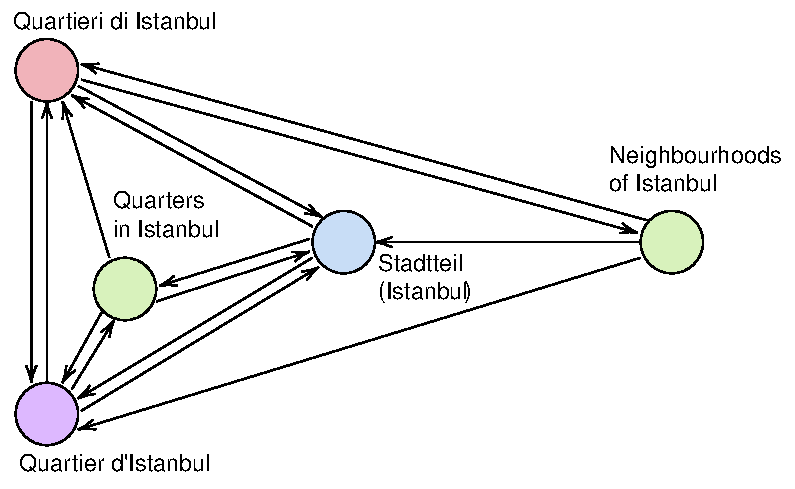
\includegraphics[width=\textwidth]{images/istanbul.pdf}
                \caption{A typical ambiguity of the Wikipedia multilingual graph built with categories and inter-language links. Different colors represent nodes belonging to different Wikipedia editions: green is used for English, red for Italian, blue for German and purple for French. Data come from the dump dated January 1st 2019. Here the confusion is given by the fact that Italian, French and German edition do not have two different categories for the English \textquote{Neighbourhoods of Istanbul} and \textquote{Quarters in Istanbul}. This is probably explained by by the fact that boundaries of concepts vary across language-defined communities.}
                \label{istanbul}
            \end{figure}
        
            The predefined merging strategy repeatedly removes a random edge from the strongly connected component, merging the vertices linked by the edge (if possible), until no further action can be taken. This process is repeated \(N\) times, and the final merging is given by the result that is more likely to happen.
        
            When I applied the merging strategy to the strongly connected components shown in pictures \ref{red_star} and \ref{istanbul} (with \(N = 1000\)), I have obtained the results described in tables \ref{results_merging_red_star} and \ref{results_merging_istanbul}. Specifically, the merging strategy has always been able to find the two obvious components.
        
            \begin{table}[h]
                \centering
                \begin{tabular}{|c|c|c|}
                    \hline
                    First component & Second component & Perc. \\ \hline \hline
                    \makecell{Étoile rouge de Belgrade\\Sportsko Društvo Crvena zvezda\\Crvena zvezda\\Roter Stern Belgrad} & \makecell{FK Étoile rouge de Belgrade\\F.K. Crvena zvezda\\Red Star Belgrade} & 86\% \\ \hline
                    \makecell{Étoile rouge de Belgrade\\Sportsko Društvo Crvena zvezda\\Crvena zvezda} & \makecell{FK Étoile rouge de Belgrade\\F.K. Crvena zvezda\\Red Star Belgrade\\Roter Stern Belgrad} & 6\% \\ \hline
                    \multicolumn{2}{|c|}{Others (\(\ge 2\) components)} & 8\% \\ \hline
                \end{tabular}
                \caption{The result of running the predefined merging strategy (with \(N=1000\)) to the strongly connected component described in figure \ref{red_star}. Most of the times, the obvious solution is found: a component represents the multi-sport club, the other represents the football club. Therefore, the merging strategy is able to find the expected solution with a probability that increases when \(N\) is large.}
                \label{results_merging_red_star}
            \end{table}
            
            \begin{table}[h]
                \centering
                \begin{tabular}{|c|c|c|}
                    \hline
                    First component & Second component & Perc. \\ \hline \hline
                    \makecell{Quartier d'Istanbul\\Quartieri di Istanbul\\Quarters in Istanbul\\Stadtteil (Istanbul)} & Neighbourhoods of Istanbul & 68\%\\ \hline
                    \makecell{Quartier d'Istanbul\\Quarters in Istanbul\\Stadtteil (Istanbul)} & \makecell{Quartieri di Istanbul\\Neighbourhoods of Istanbul} & 21\%\\ \hline
                    \makecell{Quartier d'Istanbul\\Quarters in Istanbul} & \makecell{Quartieri di Istanbul\\Neighbourhoods of Istanbul\\Stadtteil (Istanbul)} & 7\%\\ \hline
                    \multicolumn{2}{|c|}{Others (\(\ge 2\) components)} & 4\% \\ \hline
                \end{tabular}
                \caption{The result of running the predefined merging strategy (with \(N=1000\)) to the strongly connected component described in figure \ref{red_star}. Here the preferred solution found by the merging strategy is to create a component formed by the single \textquote{Neighbourhoods of Istanbul}.}
                \label{results_merging_istanbul}
            \end{table}
        
            However, I noticed that the merging strategy depends sometimes on the languages being used in the multilingual graph. For example, if one tries to merge only Italian and English nodes in the graph represented in figure \ref{istanbul}, he/she probably ends up with a result where the Italian \textquote{Quartieri di Istanbul} is merged with the English \textquote{Neighbourhoods of Istanbul} (in a graph formed by four languages, \textquote{Quartieri di Istanbul} would be merged with \textquote{Quarters in Istanbul}, as shown in table \ref{results_merging_istanbul}).
        
            Therefore, the order in which merging operations are performed does matter. Equally important (or authoritative) languages should be merged with a single operation, because their \textquote{opinions} are probably equally valid and should be given the same priority. In other words, given three languages \(A\), \(B\) and \(C\), and indicating with \(X \cup Y\) the merging of languages \(X\) and \(Y\), \(A \cup B \cup C \ne \left(A \cup B\right) \cup C\):
            \begin{itemize}
                \item When languages are merged together with a single operation, all the edges are equally important (because of the random choice): this is similar to an election in which every participant can vote their representatives.
                \item Adding language \(C\) to the already merged languages \(A\) and \(B\) is equivalent to give higher priority to votes coming from communities \(A\) and \(B\).
            \end{itemize}
    \section{Labelling Wikipedia categories}
        This section describes the different experiments I performed using Wikipedia categories. In particular, I used the learning framework described in chapter \ref{learning_framework} for training a graph-based convolutional neural network. It successfully learned how to classify each Wikipedia page into one of the eleven topics used in Negapedia (refer to section \ref{negapedia_categories} for more details). After that, I experimented with different curricula and with active learning: in both cases I achieved promising results.
        \subsection{Training a graph convolutional network}\label{experiments_gcn}
            As described in section \ref{spectralgeometriclearning}, the field of geometric learning --- i.e., the field that aims to build neural networks that can learn from non-Euclidean data --- allows to generalize classical convolutional neural networks to graphs, allowing the fusion of heterogeneous data defined on a domain structure. In general, these new methods are very different from graph embedding methods: instead of transforming a graph to a vector assuming that the connected nodes are likely to share the same labels, convolutional methods are performed on the input graph itself, with structure and features left unchanged.
            
            One of the most cited works in graph learning is a paper by \citeauthor{Kipf} \cite{Kipf}. The paper introduced the so-called \textquote{graph convolutional networks}: this architecture alleviates the risk of over-fitting on a local neighborhood of a graph and makes the architecture linear with respect to the Laplacian, simplifying the overall model complexity. Refer to section \ref{gcn} for more details.
            
            I decided to use a graph convolutional network --- hereafter called GCN --- to label the vertices of the Wikipedia category graph. I implemented the architecture described in \cite{Kipf} by using PyTorch\footnote{A Python open source deep learning platform with a rich ecosystem of tools and libraries.}\footnote{\url{http://www.pytorch.org}.}. Here are the specifications:
            \begin{itemize}
                \item I used the initialization scheme proposed in \cite{Glorot} (it brings substantially faster convergence).
                \item The optimization algorithm is Adam, proposed by \citeauthor{Kingma} in \cite{Kingma}. It is based on adaptive estimates of lower-order moments, it is computationally efficient, has little memory requirements, and is well suited for problems that are large in terms of data and/or parameters.
                \item I used the hyperbolic tangent function (also known as \emph{tanh}) as activation function for the layers of the network\footnote{\url{http://www.pytorch.org/docs/stable/nn.html\#tanh}.}. Moreover, since its outputs are in the range \((-1,1)\), I applied a softmax function\footnote{\url{http://www.pytorch.org/docs/stable/nn.html\#softmax}.} to the output of the last layer, rescaling the values so that they lie in the range \([0,1]\) and sum to \(1\).
                \item As a loss function, I decided to use the negative log likelihood loss\footnote{\url{http://www.pytorch.org/docs/stable/nn.html\#nllloss}.}. It is useful to train a classification problem with multiple classes.
            \end{itemize}
        \subsection{Hyperparameter tuning}\label{experiment_tuning}
            After the implementation of the model, I tried to train it. In order to do so, I needed to tune four main parameters: the learning rate used by the optimizer, the number of layers of the neural network, the number of neurons of each layer and the number of epochs.
            
            Training a (small) GCN model on such a dataset took a relatively long time (approximately 6--24 hours, depending on the complexity and the number of epochs). Therefore, a complete grid search (see section \ref{ml_hyper_optimization}) was not possible in this setting: it would have taken too long. Therefore I decided to use a mixed approach:
            \begin{enumerate}
                \item I started with a random search --- i.e., a technique that draws combinations of parameters randomly. Indeed, it usually outperforms grid search when the budget is low \cite{Bergstra}.
                \item I kept the most promising combination (different combinations were compared by using the accuracy computed on the evaluation dataset) and started a grid search in the small sub-region around it, refining the final result.
            \end{enumerate}
            
            Each trial was performed with the same fixed training-evaluation-test split (80\%-10\%-10\%). The labels that I used are those collected with the labelling platform. Moreover, since they were not enough, I kept some of the labels provided by the Negapedia categorization algorithm (specifically, I labeled the nodes the algorithm is less uncertain about, maintaining at the same time a balance between different classes in the training dataset). With regard to active learning, the budget was set to \(0\) in order to make the process fully automatic and to avoid any source of help coming from external resources.
            
            Here are the characteristics of the best GCNs I have found through the search of the parameter space:
            \begin{itemize}
                \item They have 3 or 4 layers (it was not possible to train networks deeper than 6 layers because computational resources were not enough). This makes sense because GCNs classify a graph node by using information coming from its neighbors that are up to \emph{number of layers} steps away from it, and the label of a Wikipedia category probably does not depend on categories which are too much far away.
                \item With regard to the number of neurons per layer, I noticed that in general performance increase when there are more neurons. Indeed, the best accuracy was achieved using 32 neurons per layer, which is also the maximum value that I was able to test with the computational resources I could use.
                \item The learning rate should be chosen in the interval \(\left[0.11,0.13\right]\), where the best solutions were found.
                \item The number of epochs was less influential. Good values were found in the range \(\left[400,600\right]\).
            \end{itemize} 
            
            It would be interesting to test networks with many more neurons on each layer, since the results seem to suggest that the best models are \textquote{wide}, and not \textquote{deep}. Moreover, one could also try to test architectures in which different layers have different numbers of neurons (in my trials, all the layers shared the same number of neurons).
        \subsection{Effects of using a bad dataset}
            While the accuracy of the trained model is very high when computed on the labeled pages provided by the Negapedia algorithm, it dramatically drops down when computed on the pages labeled manually by users of the labelling platform. Specifically:
            \begin{itemize}
                \item When one uses the less uncertain labels automatically provided by the algorithm developed by \citeauthor{Bonetti} \cite{Bonetti} (2000 examples per class, related to the pages with highest maximum value of the probability distribution), the average accuracy is approximately \(0.95\).
                \item When one measures the accuracy using more realistic data such as the ones provided through the labelling platform by the users, it drops down to \(0.63\).
            \end{itemize}
            
            Though the second value is not bad (better results can be obtained with more computational resources), one cannot ignore this problem. I identified two reasons behind this drop.
            \begin{itemize}
                \item First, since the GCN is given Negapedia data, it learns from them. But these data do not come without errors (they are automatically generated by an algorithm and not manually checked by a human). Therefore, the GCN learns also how to make the same mistakes made by Negapedia.
                \item The second reason can be found in the data provided by Negapedia: they were not uniformly spread through the entire graph, but they were grouped in few specific sub-graphs. Probably, the Negapedia algorithm classifies with high certainty many nodes close to each other. Moreover, when I measured the centrality of these nodes, they were always part of the 50th percentile: more than half of the vertices were more central then them. As a consequence, it is extremely difficult for the GCN to propagate information: it comes from few non-central points.
            \end{itemize}
            
            The solution to this problem is to find better data. The labelling platform can be of great help in this task.
        \subsection{Experiments with different curricula}\label{experiments_curricula}
            With a good model in hand, I started experimenting with curriculum learning: I compared a no curriculum setting (random ordering) with various curriculum settings, in which vertices are ordered by increasing difficulty or decreasing desirability.
            
            In particular, I experimented with two curricula:
            \begin{itemize}
                \item A curriculum in which the algorithm is presented the central nodes first (centrality is measured using the PageRank metric). Intuitively, if the model learns how to classify central nodes, information will propagate faster.
                \item A curriculum in which the algorithm is presented those categories in which there are articles that are highly visited on average. Intuitively, categories containing highly visited articles are more desirable because we want the algorithm to work most of the times.
            \end{itemize}
            
            Though much work can be done on tuning the curricula, I decided to keep the experiment very simple. First, I used four levels for each curriculum. Moreover, the number of vertices belonging to each level was also fixed (\(25\%\) of the vertices in each level). Finally, I trained each model for \(450\) epochs, dedicating an equal number of epochs to each curriculum level.
            
            \begin{figure}
                \centering
                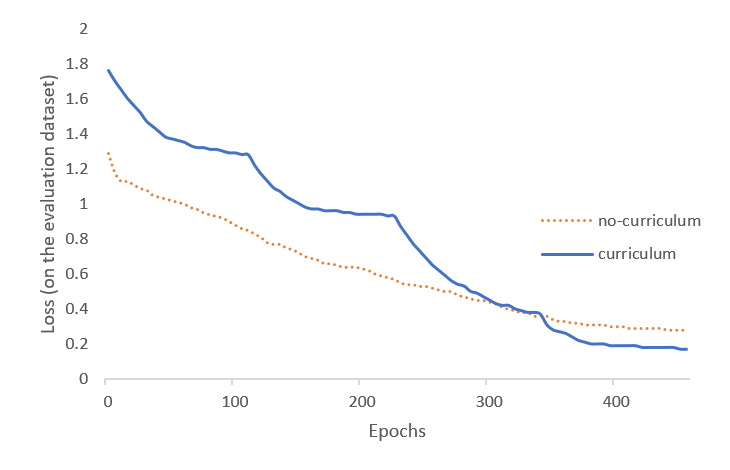
\includegraphics[width=0.8\textwidth]{images/cv_experiment.PNG}
                \caption{Comparison of two models. One does not use any curriculum, the other uses a centrality-based curriculum, in which central nodes are learned first. Both models are based on the same GCN (4 layers with 16 neurons each). For more details, refer to section \ref{experiment_tuning}.}
                \label{cv_experiment}
            \end{figure}
            
            Figure \ref{cv_experiment} shows the results that I obtained by training the model with a centrality-based curriculum. Though the loss is initially higher than in the case with no curriculum, the model rapidly improves and, in the end, it provides a better performance. The curriculum-based loss graph has the typical trend observed in \cite{Bengio}.
            
            Unfortunately, this behavior is not always achieved: if I try to use a slightly different model then sometimes the algorithm without curriculum still reaches better results. However, I want to stress the fact that I did not try to experiment with different curriculum parameters (number of epochs and instances per level, number of levels). Instead, I used some \textquote{random} values. Therefore, I think that better results can be obtained by making some changes to the parameters governing curriculum learning. This is left as future work.
            
            With regard to the visits-based curriculum, it did not achieve good (or even acceptable) results: the value of its loss function was always considerably higher than the value of the loss function of the algorithm without curriculum. This is explained by the fact that it uses desirable vertices instead of easy vertices: the goal is to learn how to classify vertices which will be used a lot by users, but they are not necessarily good for propagating information though the graph.
            
            To sum up, some curriculum strategies are likely to improve the overall training performance. Moreover, some strategies seem to work better than others. However, it is not always clear what is the best strategy and which are the vertices the model should focus on. As \citeauthor{Bengio} remarked in \cite{Bengio}, \textquote{after all, the art of teaching is difficult and humans do not agree among themselves about the order in which concepts should be introduced to pupils}.
        \subsection{Experiments with active learning}
            I also performed some experiments to understand whether using active learning is effective or not. In particular, I removed 300 random labeled vertices from the training dataset and trained the GCN model described in section \ref{experiment_tuning} with an active learning budget of 300 units. In other words, I manually labeled a vertex at each epoch for the first 300 epochs. The vertex to be labeled was chosen by the algorithm itself, using a combination of the active learning criteria (for more details, refer to sections \ref{active_learning_criteria} and \ref{combination_criteria}).
            
            \begin{figure}
                \centering
                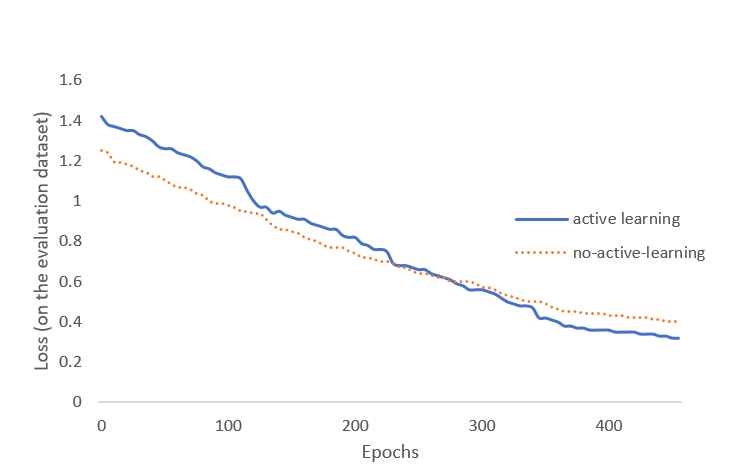
\includegraphics[width=0.8\textwidth]{images/active_experiment.PNG}
                \caption{Comparison of two models. One is trained on the entire training set (\(N\) labeled vertices), the other is trained on part of the training set (\(N-300\) labeled vertices) but it is free to query the user for 300 times. The adopted query system is the one that works with time-sensitive parameters (for a detailed description, refer to sections \ref{active_learning_criteria} and \ref{combination_criteria}). Both models are based on the same GCN (4 layers with 16 neurons each). For more details, refer to section \ref{experiment_tuning}.}
                \label{active_experiment}
            \end{figure}
            
            Then, I compared the performance of the model obtained through active learning with the performance of the model described in section \ref{experiment_tuning}. Figure \ref{active_experiment} shows the result of the experiment: it clearly shows that if the algorithm is given the freedom to choose the vertices to be labeled then the overall performance increases.
    \section{Labelling Wikipedia articles}
        Once Wikipedia categories are labeled, it is possible to label Wikipedia articles. Since I did not have enough computational resources to run a graph-based convolutional network on the entire multilingual graph of Wikipedia articles, I decided to take all the categories an article belongs to, take the average probability distribution over classes, and keep the class corresponding to the maximum value of the resulting probability distribution. An example is shown in table \ref{articles_example}.
        
\begin{table}[h]
\footnotesize
\begin{tabular}{|c||l|l|l|l|l|l|l|l|l|l|l|}
\hline
\multirow{2}{*}{Pages} & \multicolumn{11}{c|}{Classes}                                                                                                                                                                                                                                                                 \\ \cline{2-12} 
                            & \multicolumn{1}{c|}{C1} & \multicolumn{1}{c|}{C2} & \multicolumn{1}{c|}{C3} & \multicolumn{1}{c|}{C4} & \multicolumn{1}{c|}{C5} & \multicolumn{1}{c|}{C6} & \multicolumn{1}{c|}{C7} & \multicolumn{1}{c|}{C8} & \multicolumn{1}{c|}{C9} & \multicolumn{1}{c|}{C10} & \multicolumn{1}{c|}{C11} \\ \hline \hline
P1                          & 0.02                    & 0.01                    & 0.01                    & 0.03                    & 0.46                    & 0.01                    & 0.01                    & 0.02                    & 0.01                    & 0.01                     & 0.41                     \\ \hline
P2                          & 0.03                    & 0.01                    & 0.04                    & 0.06                    & 0.20                    & 0.13                    & 0.01                    & 0.08                    & 0.02                    & 0.03                     & 0.39                     \\ \hline
P3                          & 0.07                    & 0.01                    & 0.04                    & 0.06                    & 0.16                    & 0.04                    & 0.06                    & 0.01                    & 0.01                    & 0.02                     & 0.52                     \\ \hline
P4                          & 0.01                    & 0.01                    & 0.02                    & 0.01                    & 0.48                    & 0.17                    & 0.02                    & 0.01                    & 0.04                    & 0.01                     & 0.22                     \\ \hline
P5                          & 0.01                    & 0.01                    & 0.01                    & 0.02                    & 0.51                    & 0.03                    & 0.01                    & 0.04                    & 0.11                    & 0.07                     & 0.18                     \\ \hline \hline
                       Result     & 0.03                    & 0.01                    & 0.02                    & 0.04                    & \textbf{0.37}                    & 0.07                    & 0.02                    & 0.03                    & 0.04                    & 0.03                     & 0.34                     \\ \hline
\end{tabular}
\caption{Example of how an article page of the multilingual Wikipedia graph can be classified. Specifically, the example regards the \textquote{k-nearest neighbors algorithm} page of the English edition. Rows represent categories the article belong to (respectively, \textquote{Classification algorithms}, \textquote{Search algorithms}, \textquote{Machine learning algorithms}, \textquote{Statistical classification} and \textquote{Nonparametric statistics}). Columns represents the eleven labels used to categorize Wikipedia pages (from \textquote{Culture, arts and entertainment} to \textquote{Technology and applied sciences}, refer to section \ref{negapedia_categories} for more details). Each row contains the soft label --- i.e., the distribution over classes --- assigned to the related category page by the GCN model trained using the learning framework. The result is obtained by averaging values contained in each column. The highest value is \(0.37\) and corresponds to the fifth label --- i.e. \textquote{Mathematics and logic}.}
\label{articles_example}
\end{table}

        The results that I obtained by applying this simple algorithm are very promising. Indeed, I checked the labels assigned to 100 random articles belonging to the English and Italian editions and I measured an accuracy of 53\%. The value is certainly not high, but it is obtained by using a model trained on data that are probably of low quality. Moreover, this accuracy is obtained by simply using information coming from categories: I did not even try to exploit the full potential of the multilingual graph of the Wikipedia articles. For example, one could use page title or summaries, links to other articles, interests of the contributors, etc. Therefore, though this is only a basic experiment with articles, I think that it demonstrates that one could easily achieve better results by exploiting the power of the multilingual graph.